% !TEX program = xelatex
% Homework template

\documentclass[cn,12pt]{homework}
% en is for English language
% cn is for Chinese language

%----- text fonts -----
% \usepackage{newtxtext}
% \setmainfont{Times New Roman}

%----- math font -----
\usepackage{newtxmath}
\usepackage{mathptmx}
\usepackage{mathpazo}
\usepackage{listings}
\usepackage{enumitem}
\usepackage{float}
\usepackage{xcolor}
\usepackage{fancyhdr}
\pagestyle{fancy}
\lstset{
    %backgroundcolor=\color{red!50!green!50!blue!50},%代码块背景色为浅灰色
    rulesepcolor= \color{gray}, %代码块边框颜色
    breaklines=true,  %代码过长则换行
    numbers=left, %行号在左侧显示
    numberstyle= \small,%行号字体
    keywordstyle= \color{blue},%关键字颜色
    commentstyle=\color{gray}, %注释颜色
    frame=shadowbox%用方框框住代码块
    }

%----- custom theorem -----
\newtheorem{innercustomgeneric}{\customgenericname}
\providecommand{\customgenericname}{}
\newcommand{\newcustomtheorem}[2]{%
  \newenvironment{#1}[1]
  {%
   \renewcommand\customgenericname{#2}%
   \renewcommand\theinnercustomgeneric{##1}%
   \innercustomgeneric
  }
  {\endinnercustomgeneric}
}

\newcustomtheorem{ntheorem}{定理}
\newcustomtheorem{nlemma}{引理}

%----- list style -----
\setlist{nolistsep}

% differential operator
\newcommand{\dif}{\mathop{}\!\mathrm{d}}

% new command
\newcommand{\CC}{\ensuremath{\mathbb{C}}}
\newcommand{\RR}{\ensuremath{\mathbb{R}}}
\newcommand{\A}{\mathcal{A}}
\newcommand{\bA}{\boldsymbol{A}}
\newcommand{\ii}{\mathrm{i}\,}
\newcommand{\dx}[1][x]{\mathop{}\!\mathrm{d}#1}
\newcommand{\abs}[1]{\lvert#1\rvert}
\newcommand{\norm}[1]{\left\lVert#1\right\rVert}
\newcommand{\red}[1]{\textcolor{red}{#1}}

%----------------------------------------------------
%	HOMEWORK INFORMATION
%----------------------------------------------------

\lhead{\itshape Artificial Intelligence   } % 页眉
\rhead{}
\title{HOMEWORK \#1} % 作业名字

\date{Date: \today} % 日期

\institute{ZHEJIANG UNIVERSITY\quad COLLEGE OF INFORMATION SCIENCE AND ELECTRONICS ENGINEERING} % 学院或学校

\courseinfo{Artificial Intelligence } % 课程信息

\studentinfo{Name: \textit{}  \quad  \quad Student ID: \textit{}  \quad \\ Major: \textit{Electronic Science and Technology}} % 学生信息


\begin{document}

\maketitle

%----------------------------------------------------
%	作业内容
%----------------------------------------------------

%\section*{作业题目}

%------------------------------%
%------------------------------%
\begin{problem}

{\fontseries{bx}\selectfont Give a complete problem formulation for each of the following. Choose a formulation that is precise enough to be implemented.}

\begin{enumerate}[label=\alph*)]
    \item Using only four colors, you have to color a planar map in such a way that no two adjacent regions have the same color.
    \item A 3-foot-tall monkey is in a room where some bananas are suspended from the 8-foot ceiling. He would like to get the bananas. The room contains two stackable, movable, climbable 3-foot-high crates.
    \item You have a program that outputs the message ``illegal input record'' when fed a certain file of input records. You know that processing of each record is independent of the other records. You want to discover what record is illegal.
    \item You have three jugs, measuring 12 gallons, 8 gallons, and 3 gallons, and a water faucet. You can fill the jugs up or empty them out from one to another or onto the ground. You need to measure out exactly one gallon.
\end{enumerate}

\end{problem}


\begin{solution}
  \quad

  \textbf{a: Four-Color Map Problem}

  \textbf{Initial State:}  
  All regions are uncolored.

  \textbf{Successor function:}  
  Assign a color to an uncolored region, ensuring that the chosen color is different from the colors of all adjacent regions.

  \textbf{Goal Test:}  
  All regions are colored, and no two adjacent regions share the same color.

  \textbf{Cost Function:}  
  Assume the cost of coloring a region is 1. The total cost is the number of regions, \(n\).
  \newline

  \textbf{b: Monkey and Bananas Problem}

  \textbf{Initial State:}  
  The monkey is on the ground, the two crates are on the ground, and the bananas have not been reached:

  \textbf{Successor function:}  
  1. Move the monkey to a crate or the ground.
  2. Move a crate to a new position.
  3. Stack one crate on top of the other.
  4. Unstack one crate from the other.
  5. Climb a crate.
  6. Grab the bananas.

  \textbf{Goal Test:}  
  The monkey reaches the bananas:

  \textbf{Cost Function:}  
  Assume each action has a cost of 1. The total cost is the number of actions taken to reach the goal.
  \newline

  \textbf{c: Illegal Input Record Problem}

  \textbf{Initial State:}  
  The full set of input records.

  \textbf{Successor function:}  
  1. Divide the current set of records into smaller subsets.  
  2. Test each subset to determine if it contains the illegal record.  
  3. Discard subsets that do not contain the illegal record.

  \textbf{Goal Test:}  
  Find the single illegal record.

  \textbf{Cost Function:}  
  The cost is the number of tests performed. The goal is to minimize the number of tests.
  \newline

  \textbf{State Space:}  
  Each state represents the amount of water in the three jugs. A state can be represented as a tuple \((x, y, z)\), where:
  - \(x\): The amount of water in the 12-gallon jug.
  - \(y\): The amount of water in the 8-gallon jug.
  - \(z\): The amount of water in the 3-gallon jug.

  \textbf{Initial State:}  
  \((0, 0, 0)\), where all jugs are empty.

  \textbf{Successor function:}  
  1. Fill a jug completely from the faucet.  
  2. Empty a jug onto the ground.  
  3. Pour water from one jug into another until either the first jug is empty or the second jug is full.

  \textbf{Goal Test:}  
  The goal is to measure exactly 1 gallon of water in any of the jugs. For example, a goal state could be \((1, y, z)\), \((x, 1, z)\), or \((x, y, 1)\).

  \textbf{Cost Function:}  
  Assume each action has a cost of 1. The total cost is the number of actions taken to reach the goal.

\end{solution}
%------------------------------%
\newpage
\begin{problem}

{\fontseries{bx}\selectfont Consider a state space where the start state is number 1 and each state khas two successors: numbers 2k and 2k + 1.}

\begin{enumerate}[label=\alph*)]
    \item Draw the portion of the state space for states 1 to 15.
    \item Suppose the goal state is 11. List the order in which nodes will be visited for breadth-first search, depth-limited search with limit 3, and iterative deepening search.
    \item How well would bidirectional search work on this problem? What is the branchingfactor in each direction of the bidirectional search?
    \item Does the answer to (c) suggest a reformulation of the problem that would allow you tosolve the problem of getting from state 1 to a given goal state with almost no search?
    \item Call the action going from k to 2k Left, and the action going to 2k + 1 Right. Can youfind an algorithm that outputs the solution to this problem without any search at all?
\end{enumerate}

\end{problem}

\begin{solution} 
  \quad

  \textbf{a: The figure of the state space for states 1 to 15 is shown below:}

  \begin{figure}[H]
    \centering
    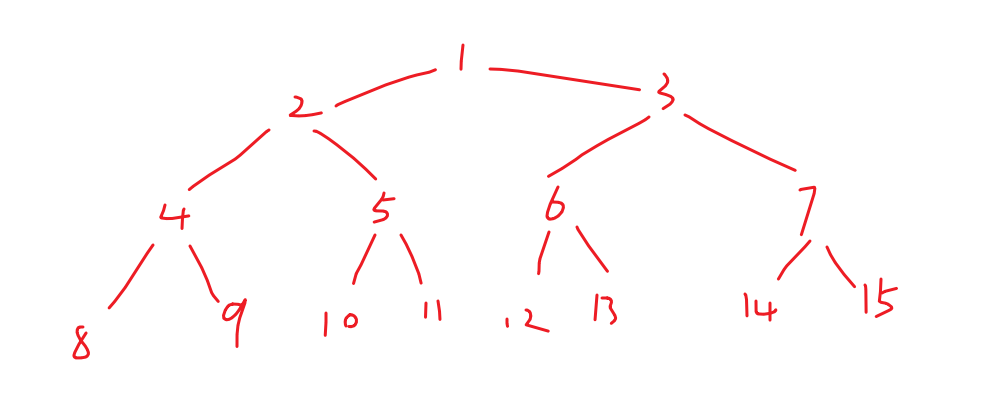
\includegraphics[width=0.8\textwidth]{figures/image1.png}
    \caption{State Space for States 1 to 15}
  \end{figure}

\textbf{b: The order in which nodes will be visited for each search method is as follows:}

  BFS Order: \(1, 2, 3, 4, 5, 6, 7, 8, 9, 10, 11\).

  Depth-Limited Search with limit 3 Order: \(1, 2, 4, 8, 9, 5, 10, 11\).

Iterative Deepening Search Order:  

  Depth 0: \(1\)  

  Depth 1: \(1, 2, 3\)  

  Depth 2: \(1, 2, 4, 5, 3, 6, 7\)  

  Depth 3: \(1, 2, 4, 8, 9, 5, 10, 11\).

\textbf{c: }

  Bidirectional search work well on this problem because the goal state is known. In the reverse direction, the successors of a state \(n\) are \(\lfloor n/2 \rfloor\),only one successor,so it is easy to find the path from the goal state to the start state.

  The branching factor in forward direction is 2 and in reverse direction is 1.

\textbf{d: }

Yes, start from the goal state and apply the reverse actions (Left and Right) to reach the start state. This way, the problem of getting from state 1 to a given goal state can be solved with almost no search.

\textbf{e:}

Yes, the solution can be found without search by using the binary representation of the goal state. The algorithm is as follows:

1. Convert the goal state \(k\) into its binary representation.

2. Starting from the second bit (ignoring the leading 1), interpret each bit:

  \(0\): Take the "Left" action.

  \(1\): Take the "Right" action.

3. Output the sequence of actions.

\end{solution}

\newpage

\begin{problem}

{\fontseries{bx}\selectfont Consider the two-player game described in Figure 5.17}
  \begin{figure}[H]
    \centering
    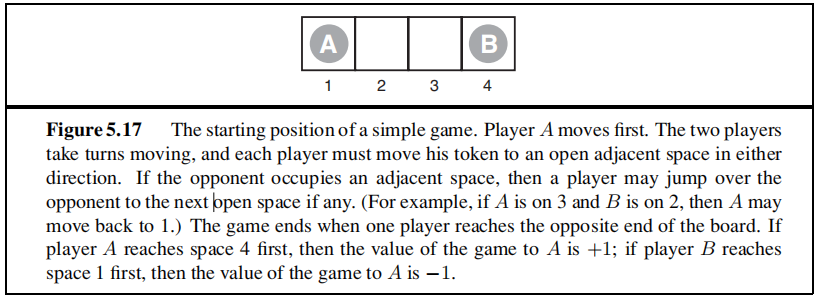
\includegraphics[width=0.8\textwidth]{figures/image2.png}
    \caption{figure 5.17}
  \end{figure}
\begin{enumerate}[label=\alph*)]
    \item Draw the complete game tree, using the following conventions:
    \begin{itemize}
        \item Write each state as \((s_A, s_B)\), where \(s_A\) and \(s_B\) denote the token locations.
        \item Put each terminal state in a square box and write its game value in a circle.
        \item Put loop states (states that already appear on the path to the root) in double square boxes. Since their value is unclear, annotate each with a "?" in a circle.
    \end{itemize}
    \item Now mark each node with its backed-up minimax value (also in a circle). Explain how you handled the "?" values and why.
    \item Explain why the standard minimax algorithm would fail on this game tree and briefly sketch how you might fix it, drawing on your answer to (b). Does your modified algorithm give optimal decisions for all games with loops?
    \item This 4-square game can be generalized to \(n\) squares for any \(n > 2\). Prove that A wins if \(n\) is even and loses if \(n\) is odd.
\end{enumerate}


\end{problem}

\begin{solution}

  \quad

\textbf{a:} The complete game tree is shown below:

\textbf{b:} 

If all the successors have "?" values,it's obvious that the parent node will also have a "?" value. 

Otherwise, the backed-up minimax value of a node is the maximum value of its successors if it is a MAX node, and the minimum value of its successors if it is a MIN node.


  \begin{figure}[H]
    \centering
    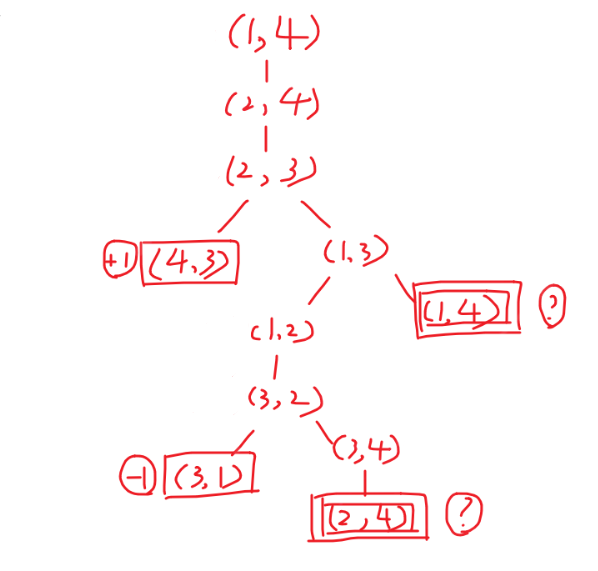
\includegraphics[width=0.7\textwidth]{figures/image4.png}
    \caption{Game Tree}
  \end{figure}

    \begin{figure}[H]
    \centering
    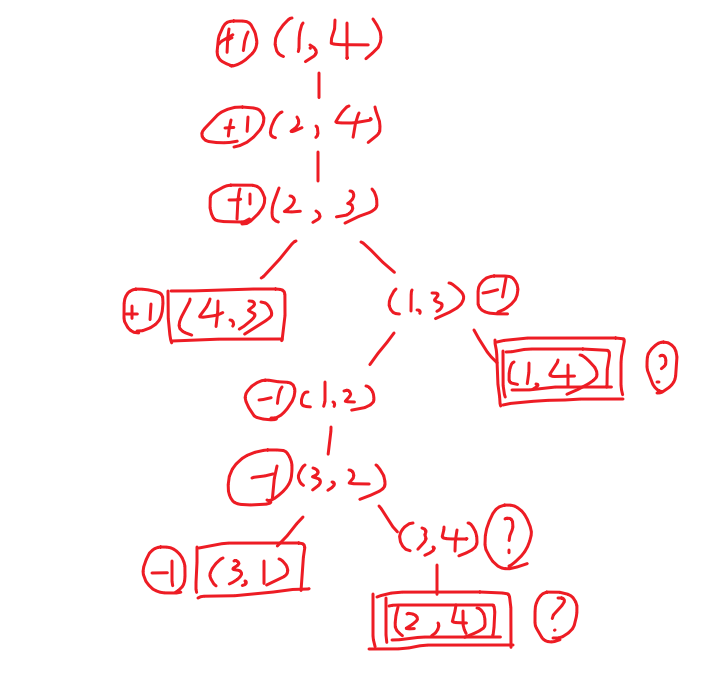
\includegraphics[width=0.7\textwidth]{figures/image3.png}
    \caption{complete game tree}
  \end{figure}



\textbf{c: }



1.The standard minimax algorithm fails on this game tree because it does not account for loops. When a loop is encountered, the algorithm may enter infinite recursion or fail to assign a value to the loop state.

2.To handle loops, the algorithm must detect repeated states and assign them a value based on the minimax principle:
  \begin{itemize}
  \item Use a visited set to track states that have already been evaluated.

  \item When a loop is detected, assign a "?" value 

  \item handled the “?” values as (b) described.
  \end{itemize}

3.The modified algorithm provides optimal decisions for games with loops as long as the loop values are assigned consistently based on the minimax principle. However, the solution may not be optimal if the loop values are not well-defined or if the game has stochastic elements.



\textbf{d: }

We can prove this by induction on \(n\):

Base case: \(n = 3\), A loses. This can be verified by examining the game tree.

Inductive step: Assume when \(n = 2k+1\)  (k>1) , A loss

When \(n = 2k+3\), it is [1,2,3 ··· ,2k+3]. At first A in 1 and only move to 2,B in 2k+3 and only move to 2k+2. Now it begin a subgame in [2,3 ··· ,2k+2].
According to the induction hypothesis, A loss in [2,3 ··· ,2k+2]. So no matter how A move, B can always move to 2 before A move to 2k+2. When B in 2, if A not in 1, B win with move to 1. If A in 1, B win with move to 3,A to 2 , B to 1.

Thus if when \(n = 2k+1\)  (k>1) , A loss.Then A also loss when \(n = 2k+3\). According to the induction, A loss when \(n\) is odd.

Same as above, when \(n = 4\), A wins. It can be verified by examining the game tree.

Similarly, we can prove that when \(n = 2k+2\) (k>1), A wins.

Above all, A wins if \(n\) is even and loses if \(n\) is odd.

\end{solution}
%------------------------------%


\newpage




\begin{problem}

{\fontseries{bx}\selectfont Consider the problem of solving two 8-puzzles.}
\begin{enumerate}[label=\alph*)]
    \item How large is the reachable state space? Give an exact numerical expression.
    \item Suppose we make the problem adversarial as follows: the two players take turns mov-ing; a coin is flipped to determine the puzzle on which to make a move in that turn;and the winner is the first to solve one puzzle. Which algorithm can be used to choosea move in this setting?
    \item Give an informal proof that someone will eventually win if both play perfectly.
\end{enumerate}


\end{problem}


\begin{solution}

  \quad

\textbf{a:}

For a single 8-puzzle, the total number of possible arrangements of the 9 tiles (8 numbered tiles and 1 blank space) is \(9!\). However, only half of these arrangements are solvable, so the reachable state space for a single 8-puzzle is:
\[
\frac{9!}{2} = 181,440
\]

For two independent 8-puzzles, the state space is the Cartesian product of the state spaces of the two puzzles. Therefore, the total reachable state space is:
\[
\left(\frac{9!}{2}\right)^2 = 181,440^2 
\]

\textbf{b: }

In this case, the random nature of the game makes it a stochastic game. 
The algorithm that can be used to choose a move in this setting is the \textbf{Expectiminimax algorithm}. 

\textbf{c:}

For the Initial two 8-puzzles, it is Non-competitive game, and the two players can play perfectly to solve they own puzzle, the state space is finite and ever player make the best move, the game will eventually end.


But for the two-player adversarial 8-puzzle game in (b), the game is competitive and stochastic. The game may not finish.

consider the following:

A player toss a coin to determine he can move in the 1st puzzle and the 1st puzzle will be solved with 2 moves. 
In this case, if A choice to move towards the goal, we can calculate the probability of A win is 1/3 and B win is 2/3(1/2+1/8+1/32+...=2/3).

So,in this case, by the Expectiminimax algorithm, A should not move towards the goal.

In order to finish the game, it always come with the case shown below, and the perfectly play will not choice to move towards the goal. So, the game will not  eventually end.



\end{solution}

















%------------------------------%
\end{document}

